% --------------------------------------------------------------------

\section{Johdanto}



\subsection{Johdantoluku}

Tämä kandinaatintyö käsittelee eletunnistusta Kinect syvyyskameran avulla. 
Työn tarkoitus on tutustua erilaisiin eletunnistusmenetelmiin ja erityisesti ChalearnChallenge kilpailun kilpailutöihin. \\

Kuvaa ja videokuvaa on tutkittu paljon, mutta eletunnistus on edelleen suuri haaste. Kehittynyt tekniikka
kuten Microsoftin Kinect -sensori ja suuri laskentateho tuovat kuitenkin uusia mahdollisukksia. 
Kinect sensori tarjoaa ns. 3D -videokuvaa eli tavallisen värikuvan lisäksi Kinect -kamera antaa infrapunakameralla mitattua syvyyskuvaa.\\

Lisätäkseen kiinnostusta 3D-kuvaan järjestettiin ChaLearn challenge eletunnistuskilpailu, joissa kilpailijat kehittivät Kinect sensorin datalle suunnattuja 
eletunnistus menetelmiä. Tämä kandinaatin työ tutustuu kilpailutöihin ja kartoittaa niiden avulla alan uusinta tutkimusta. \\



\section{Eletunnistus videokuvalta}
\label{Eletunnistus videokuvalta}


\subsection{Eletunnistus ongelmana}
Eletunnistuksella tarkoitetaan tässä työssä ihmisen suorittaman eleen tunnistamista videokuvalta. Eleitä voisivat olla esimerkiksi
viittomakielen eleet tai yksinkertaiset toiminnot kuten istuminen. Eletunnistus on haastava ongelma. Ihmisen eleet ovat usein 
monimutkaisia ja videokuvalla on paljon muuttujia kuten valaistus, tila tai kohteen etäisyys kamerasta.\citep {1251144} Eletunnistus on hyvä erottaa
asennon tunnistus (Pose Estimation) -ongelmasta. Asennon tunnistuksessa pyritään tunnistamaan henkilön asento videolla yhdessä pysäytyskuvassa
käyttämättä lainkaa ajallista tietoa. (x-box artikkeli) Yksittäisiä asentoja voidaan käyttää tunnistamaan ele, joskin se on laskennallisesti raskasta.\\

Kiinnostus eletunnistusta kohtaan on lisääntynyt viime vuosina sen monien käyttötarkoitusten vuoksi.
Parantunut laskentateho ja halvat syvyyskamerat luovat uusia mahdollisuuksia.\citep {6239178}
Eletunnistusta voidaan käyttää esimerkiksi elekäyttöliittymissä. \citep {1251144} Yksittäisiä eleitä voidaan käyttää esimerkiksi kodinkoneiden ohjailuun. Toisaalta eleentunnistusta voidaan käyttää hyödyksi tunnistamaan
erilaisia vaaratilanteita. Esimerkiksi potilaan tilaa voidaan seurata eletunnistuskameralla mahdollisten poikkeavien eleiden varalta.
\\

Videokuvan tunnistuksessa voidaan hyödyntää perinteisiä hahmontunnistusmenetelmiä. Monet menetelmistä ovat laskennallisti liian raskaita 
reaaliaikaseen videokuvan tunnistukseen. \citep {1251144} Monet hahmontunnistusmenetelmät vaativat myös paljon opetusdataa. Kuluttajille suunnatuissa
sovelluksissa olisi toivottavaa, että uuden eleen voi opettaa muutaman testinäytteen perusteella \citep {1251144}.\\

Eletunnistuksessa, kuten hahmontunnistuksessa usein, pyritään matkimaan ihmisen toimintamalleja. Käytännössä huimaa vauhtia kehittynyt tekniikka on kuitenkin
viime aikoina ajanut tutkimuksen ohi ja monet menetelmät on kehitetty nopeasti lähinnä vastaamaan käytännön tarpeisiin ja tämä näkökulma on unohdettu. (Results and Analysis of the ChaLearn Gesture Challenge 2012)


\subsection{Eletunnistus video ja 3D-videokuvalta}

Eleentunnistus videokuvalta koostuu tyypillisesti seuraavista vaiheista. Aluksi videokuvaa esikäsitellään eli siitä poistetaan häiriötä tai kuvaa esimerkiksi 
pienennetään laskennan helpottamiseksi. Eletunnistuksen tapauksessa esikäsittelyssä pyritään usein myös erottamaan ihmishahmo taustasta. Tämä on haastavaa sillä
ihmishahmo ei välttämättä erotu esimerkiksi väritykseltään taustasta. Kinectin syvyyskameran avulla tämä onnistuu kuitenkin luotettavasti.
Videolle suoritetaan usein myös jonkinlainen ajallinen jako. Videokuva jaetaan osioihin, joiden sisällä ei ole suurta vaihtelua pysäytyskuvien välillä. Videopätkät saatetaan 
tiivistää yksittäiseen kuvaan tai niitä voidaan käsitellä pysäytyskuva kerrallaan. Jako voi tapahtua myös luokitteluprosessin aikana tai 
sitä ei välttämättä ole ollenkaan.\\

Hahmontunnistuksessa ratkaiseva vaihe on usein oikeiden piirteiden valinta. Videokuvasta voidaan tutkia esimerkiksi 
tietyn suuntaista liikettä ajan funktiona. Pysäytyskuvista voidaan arvioida kontrastivaihteluita ja sitä kautta hahmottaa viivoja tai muotoja kuvassa.
Valitut piirteet riippuvat siitä käsitelläänkö videokuvaan kokonaisuutena vai tarkastellaanko pysäytyskuvia. Piirrevalinnassa voidaan 
myös yhdistellä molempia näkökulmia. Yksittäisistä pysäytyskuvista voidaan valita kiinnostavat pisteet tutkimalla videokuvalla tapahtuvaa liikettä \citep {6239185}. \\

Tunnistusvaiheessa annettuja näytteitä verrataan opetusdatan kuvaamiin luokkiin. Tunnistusmenetelmässä huomioidaan videon aikaulottovuus.
Jos videokuvaa käsitellään yksittäisten kuvien esimerkiksi liikekuvan avulla, kuvia voidaan vertailla tavanomaisilla menetelmillä.
Jos videokuva kuitenkin esitetään yksittäisillä pysäytyskuvilla on tunnistuksessa käytettävä jonkinlaista rakenteellista mallia kuten 
Markovin muuttujaa \citep. Tässäkin voidaan yhdistellä molempia näkökulmia. 



\section{ChaLearn Gesture Challenge -kilpailu}
\label{ChaLearn Gesture Challenge -kilpailu}

\subsection{Kilpailun esittely}
ChaLearn Gesture Challenge kilpailun tarkoituksena oli lisätä kiinnostusta eletunnistukseen syvyyskameroilla.
Kilpailu alkoi vuoden 2012 aikana ja se päättyi alkuvuonna 2013.
Kilpailussa tarjottiin tietokanta, joka sisälsi 50 000 Kinect-sensorilla kuvattua videonäytettä. Videonäytteet sisälsivät yksittäisiä
eleitä esimerkiksi viittomia tai poliisin käsimerkkejä. Kilpailijoiden tarkoitus oli kehittää eletunnistusmenetelmä, jonka avulla eleet
opitaan yhdestä opetusnäytteestä. Eleitä oli jaettu kategorioihin käyttötilanteen mukaan esimerksi poliisin käsimerkit olivat yksi kategoria. Eleet joilla kilpailutöitä
testattiin olivat eri eleitä kuin opetusdatassa mutta samoista kategorioista.  \\

Videonäytteillä esiintyi aina yksi ihminen kerrallaan suorittamassa tiettyä elettä. Kuva rajatttiin yläruumiiseen ja eleet tehtiin
pääasiallisesti käsillä. Liikkeet lopetettiin ja aloitettiin aina samasta lepoasennosta. Videonäytteet sisälsivät syvyyskamerakuvan sekä värikuvan 
mutta ei ranganseurausta. Haasteita toivat vaihtelevat taustat ja valaistukset videoilla. \\

Kilpailijoille jaettiin kolme datajoukko: kehitysdata, validointidata ja lopullinen arviointidata. Dataa oli luokiteltu kategorioihin sen mukaan
oliko kyseessä esimerkiksi viittoma, luonnollinen ele vai tanssiasento. Opetusdatan näytteille tarjottiin oikeat ratkaisut.
Kilpailun loppupuolella paljastettiin lopullinen testidata jonka avulla tuloksia arvioitiin.
\citep {6239178} \\


\subsection{Katsaus kilpailutöihin}
\subsubsection {Ensimmäinen kierros}
Kilpailijoiden metodeja selvitettiin ensimmäisen kierroksen jälkeen lyhyellä kyselyllä, johon vastasi 20 ryhmää 22 parhaan ryhmän joukosta.
Vastauksista kävi ilmi, että lähes kaikki tiimit tekivät jonkinlaista kuvien esikäsittelyä. Kuvista poistetiin häiriötä, asiaanliittymättömiä 
kohteita tai tausta. Huomioitavaa on kuitenkin, että jotkin hyvin menestyneistä ryhmistä eivät tehneet minkäänlaista esikäsittelyä kuville.\\

Suurin osa osallistujista käytti HOG/HOF - piirteitä \citep {}, SIFT/STIP piirteitä \citep {}, kulmien tai nurkkien tunnistusta tai kehitti omia tälle datalle 
soveltuvia ominaisuuksia. Piirteitä saattettiin tunnistaa yksittäisistä pysäytyskuvista tai jonkinlaisista summakuvista.
Suurin osa kilpailijoista käytti tunnistustuksessa pelkkää syvyyskuvaa, osa molempia, sekä väri- että syvyyskuvaa. 
Mielenkiintoista on, että toisen sijan voittaja käytti työssään pelkkää RGB-videokuvaa. 
Kilpailijat käyttivät kaikki jonkilaista piirteiden tiivistystä tai kuvausta toiseen lineaariavaruuteen.\\

Videokuvaa jaettiin ajallisesti osioihin perustuen videokuvan samankaltaisuuteen. Ajallisen rakenteen mallintamiseen käytettiin erilaisia graafisia malleja
kuten Hidden Markov Model ja Conditional Random Fields. Itse luokittelu tapahtui k-lähimmän naapurin luokittimella tai muilla yksinkertaisilla keinoilla. 
Kilpailun järjestejien odottamaa metodia Transfer learning käytettiin vähäisesti, eikä kukaan menestyneistä kilpailijoista ei käyttänyt sitä. \\
\citep {6239178} 

Kahdeksan menestyneintä työtä löytyy taulukosta ~\ref{table:dvbt_param}. Seuraavassa luvussa esitellään kolme menestyneistä töistä tarkemmin.
Työt ovat eräitä esimerkkejä toimivista ratkaisuista. Ne on valittu tähän, koska ne edustavat erilaisia näkökulmia ongelmaan. Valintamahdollisuuksia
rajoitti se, että kaikki kilpailijat eivät olleet vielä julkaisseet menetelmäänsä tämä työn kirjoittamisen aikana.\\\

\begin{table}[th]
\caption{ChaLearn Challenge kahdeksan parhaiten sijoittunutta ryhmää}
\label{table:dvbt_param}
\begin{center}
\begin{tabular}{|p{0.35\textwidth}|p{0.45\textwidth}|} 
    \hline
Ryhmän nimi & Menetelmä \\
    \hline
    \hline
alfnie & Motion Signature analyses\\ 
    \hline
Pennect & HMM-style method using HOG/HOF features
with a temporal segmentation based on candidate cuts.
Only RGB images were used.\\
    \hline
One Million Monkeys & HMM\\
    \hline
immortals & HOG/HOF features\\
    \hline
Zonga & Least Squares Regression, HOSVD\\
    \hline
Balazs Godeny & Thumbnail Dynamic Time Warping” (DTW).\\
    \hline
SkyNet & Dynamic Time Warping(DTW)\\
    \hline
xiaozhuwudi & MHI by adding GEI and INV\\
    \hline	
\end{tabular}
\end{center}
\end{table}

\subsubsection {Toinen kierros}
\newpage
\section {Katsaus menestyneisiin kilpailutöihin}

\subsection{xiaozhuwudi ja laajennettu MHI}
Ryhmä xiaozhuwudi lähti liikkeelle MHI eli Motion History Image -tekniikasta. \citep {6239179} MHI tutkii liikkeen määrää videokuvalla.
Videopätkä tiivistetään yhteen liikekuvaan, joka kuvaa liikkeen viimeaikaisuutta. Kohdat, joissa videokuvalla on ollut
liikettä esitetään harmaasävyillä. Mitä viimeaikasempaa liike on ollut sitä valkoisempana se näkyy kuvassa. Liikkumattomat
alueet näkyvät täysin mustana. Videokuvalta tutkitaan siis vain liikettä, eikä pyritä esimerkiksi tunnistamaan kuvalla olevia kohteita
tai ihmiskehon osia. Tämä menetelmä matkii ihmisen tapaa tunnistaa eleitä. Ihminen tunnistaa erittäin hyvin inhimilliset eleet  
sumealtakin videokuvalta vaikka ei yksittäisestä framesta tunnistaisi edes ihmishahmoa. \citep {910878}  \\
\begin{figure}[htb]
  \begin{center}
    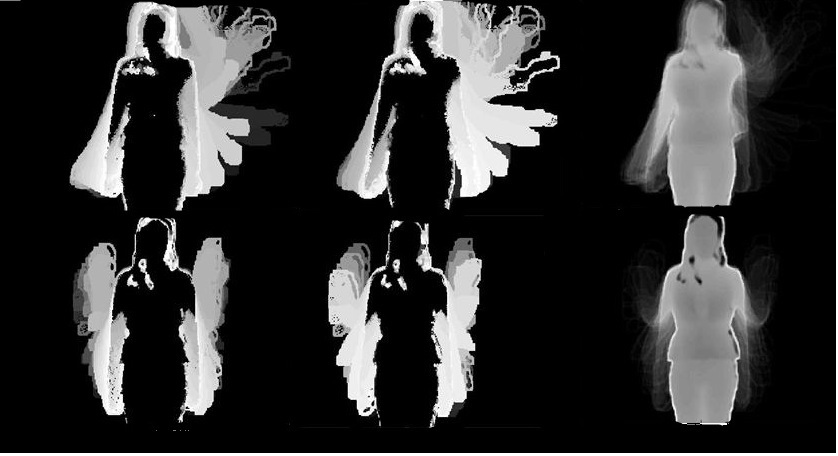
\includegraphics[width=0.4\textwidth]{mhi_ex.jpg}
    \caption{Kuvassa vasemmalta oikealle MHI, INV ja MEI. \citep {6239179}}
    \label{fig:mhiinvmei}
  \end{center}
\end{figure}
Xiaozhuwudi-ryhmä tunnistaa MHI:ssa kuitenkin ongelmia. MHI ei tunnista kovin hyvin eleitä, jotka sisältävät toistuvaa liikkeitä esimerkiksi vilkutusta.
Liikkeen toistuessa MHI -kuva muuttuu helposti sekavaksi ja on vaikea erottaa tarkkaa liikerataa. Xiaozhuwudi ehdottaa MHI:n laajentamista INV ja GEI -kuvilla.
INV oon käänteinen kuvaus MHI:ille. INV:ssa katsotaan videokuvaa alusta loppuun päin.
Mitä aikasemmin liike esiintyy videolla sitä vaalempana se näytetään kuvassa. INV:n avulla saadaan kuvaus videon alkutilanteesta, mikä täydentää MHI kuvaa. 
GEI-kuva esittäää liikkeen määrää keskimäärin koko videon aikana. Siinä summataan koko videon liike yhdelle kuvalle ja jaetaan lopuksi koko aikavälille.
GEI muistuttaa MEI:tä (Motion Energy Image), jossa myös lasketaan liikkeelle summa. Voidaan ajatella että siinä missä MHI ja INV mittaavat liikettä 
MEI ja GEI mittaavat energiaa, joka on kulunut liikkeeseen. GEI:n avulla liikkeestä saadaan hyvä kokonaiskuva ja se on hyödyllinen etenkin toistuvan
liikkeen tunnistuksessa. \citep {6239179} Katso tarkemmin kuvasta  ~\ref{fig:mhiinvmei}. \\

Datan esikäsittelyssä xiaozhuwudi hyödynsi Kinectin syvyyskuvaa poistamalla taustan ihmishahmolta. Lisäksi esikäsittelyssä poistettiin häiriöitä.
MHI, GEI ja INV -kuville suoritettiin dimensioiden vähennys. Eleiden tunnistukseen käytettiin Maximum Correlation Coeffient -luokittelijaa. \citep {6239179}\\

xiaozhuwudi sijoittui kilpailussa kahdeksannelle sijalle. 



\subsection{immortals ja Hidden Markov Model}

Ryhmä Immostals lähti kilpailutyössään liikkeelle oletuksesta, että ele koostuu ennen kaikkia useista yksittäisistä liikkeistä. 
Sen mukaan eleet tunnistetaan parhaiten käsittelmällä elettä jokkona liikkeitä. Tämä eroaa ryhmän mukaan tyypillisestä 
tavasta lähestyä ongelmaa.\\

Ryhmä lähti liikkeelle opetusvaiheessa yksittäisistä liikkeistä. Yksittäisille liikkeille luodaan allekirjoitus eli malli,
jonka avulla ne voidaan tunnistaa. Allekirjoituksen luominen on monivaiheinen operaatio. Ensin kuvista poimitaan niin sanotut
tärkeät pisteet eli pisteet joilla on merkitystä liikkeen tunnistamisen kannalta. Tässä Immortals hyödynsi Kinectin syvyyskuvaa.
Immortals arvioi, että ne kohdat kuvasta joissa on tapahtunut muutosta syvyyskameran kuvassa ovat kyseisen videon pysäytyskuvan
tärkeitä pisteitä. Tämän jälkeen tärkeille pisteille lasketaan HOG (Histogram of oriented gradients) ja HOF (Histogram of Flow). 
Kuva jaetaan pieniin alueisiin, joissa tarkastellaan alueen värityksen intensiteettivaihtelua.
Alueelle lasketaan intensiteettivihtelun gradienttien suuntien histogrammi. Ajatuksen on päätellä minkä suuntaisia 
viivoja alueelta voidaan erottaa. Tämän jälkeen histogrammit ryhmitellään tavallisen ryhmittelyalgoritmin avulla.
Histogrammeja kutsutaan tässä "visuaalisiksi sanoiksi". Tarkoituksena on tutkia sanojen esiintymistä yhdessä ja muodostaa niistä aihepiirejä. 
Yksittäistä pysäytyskuvaa voidaan kuvata sillä, mitä sanoja ja mistä aihepiireistä esiintyy siinä.\\

Liikkeelle luodaan sanojen perusteella perusteella malli, jota käytetään tunnistusvaiheesa. Mallin perustana on Markovin muuttuja
eli HMM (Hidden Markov Model). Malli kertoo kuinka todennäköisesti annettu havainto kuuluu kuvaamansa luokkaan. 
Ajatuksena on, että annetun havainnon malli on tuntematon, mutta voimme löytää etsimällä todennököisimmän mallin.
Koska tutkitaan kahta piirrettä, HOG ja HOF, käytetään monikanavaista Markovin piilomallia eli McHMM. 
HOG ja HOF piirteet paljastavat erilaista tietoa havainnosta ja tukevat tässä hyvin toisiaan.\\

McHMM parametreja ovat alkutila, todennäköisyys tilojen väliselle muutokselle sekä tilan todennäköisyys ja tilan kuvaus visuaalisten sanojen avulla. 
Tilalla tarkoitetaan tässä yksittäistä pysäytyskuvaa. Kyseessä on Bayesiamlainen menetelmä: jakauma tunnetaan, mutta ei parametreja.
Parametrien arvot optimoidaan niin, että todennököisyys opetusliikkeelle kuulua kuvaamaansa luokkaan on mahdollisimman suuri.\\
tähän joku kaava? \\

Tunnistusongelma pelkistyy lopulta kysymykseen: Mikä liikejoukko kaikken todennäköisimmin on muodostanut tämän videon?
Tämän tyylinen ongelma voidaan ratkaista Viterbin algoritmillä. Tämä vaatii kuitenkin, että ele rajataan koostumaan tietystä määrästä liikkeitä.
Kilpailussa on määritelty, että jokainen elenäyte sisältää viisi liikettä.
Viterbin alkorytmi pyrkii löytämään todennököismmän polun eri liikkeiden välillä. Alkorytmi käy videota läpi liike kerrallaan ja laskee mikä
on mallien perusteella mikä on todennäköisin liike. Lopuksi saadaan todennököisin liikesarja josta ele koostuu.
Liikesarja voidaan tunnistusvaiheessa liittää tiettyyn eleeseen. \citep {6239185}\\ 


\subsection{Zonga ja pieninimmän neliösumman menetelmä sovelluttuna monistoon}
Ryhmä Zonga käyttää kehittämäänsä menetelmää, joka soveltuu yleisesti videokuvan luokitteluun. 
Menetelmää on kuitenkin kustomoitu eletunnistusta varten tähän haasteeseen.\\

Videonkuvan käsittelyssä ensimmäinen tehtävä on usein kuvata videokuva vektoriksi tai tensoriksi, joka voidaan esittää tila-avaruudessa. 
Videokuva ei ole lähtökohtaisesti piste Euklidisessa avaruudessa, vaan monimuotoinen datajoukko. Avaruudessa olevia pisteitä voidaan käsitellä
ja esimerkiksi luokitella yksinkertaisten algoritmien avulla.\\

Ryhmä Zonga ehdottaa videon kuvamista pisteenä Grassmannin monistossa. Videokuvan kolme ulottuvuutta (leveys, korkeus ja aika) ovat moniston ulottuvuudet.
Monisto säilyttää alkuperäisen havainnon geometrisen rakenteen paremmin kuin Euklidinen avaruus.
Havainnon alkuperäinen rakenne usein kadotetaan muissa eletunnistusmenetelmissä. \\

Monistojen käyttäminen ei ole kuitenkaan täysin uusi asia eletunnistuksessa.
Ryhmä Zonga yhdistää kuitenkin monistoihin pienimmän neliösumman menetelmän, mikä tekee ryhmän tekniikasta ainutlaatuisen. 
Video on tyypillisesti kolmiulottoinen tensori, joten on luonnollista käsitellä sitä monistossa.
Pienimmän neliösumman menetelmä on regressio-ongelma, eli etsinään jonkinlaista suhdetta havainnon ja luokan välille.
Regressio-ongelma on tyypillisesti muotoa y = A * beta, jossa y -vektori esittää pisteet tulosavaruudessa, A on havaintomatriisi 
ja b -vektori on painovektori, joka kuvaa havaintomatriisin pisteet tulospisteiksi.
Meillä on siis opetusvaiheessa käytössä havainto ja sitä vastaava luokka joiden välille kehitän funktio.\\

Pienimmän neliösumman menetelmässä pyritään minimoimaan luokitteluvirheen neliötä eli oikean tulokset ja arvioidun tuloksen erotuksen neliötä.
Minimoidaan siis funktiota: \\
R(beta) = ||y-A*beta|| \\
jolloin b:lle saadaan funktio\\
funktio tähän\\

Havaintomatriisi A muodostetaan kolmesta tekijästä: videon korkeussuuntaisesta kuvaajasta, leveyssuuntaisesta sekä ajallisesta vaihtelusta.
Havaintomatriisin luomisessa käytetään HOSVD:ia. Painovektori b kuvaa havaintomatriisin A vektoriavaruuteen, missä kadotetaan tieto alkuperäisistä tekijöistä. 
Lopullista regressiota varten halutaan kuintenkin palauttaa pisteet havainnon tekijöihin.
Näin luokittelussa huomioidaan alkuperäisen havainnon rakenne ja vastataan eletunnistusongelmaan tehokkaammin. 
Lopullinen regressio kaava on siis muotoa\\
tähän se lopullinen kaava pisteen kera\\
Pistefunktio on operaatio joka kuvaa havainnot Grasmanin monistossa. Grasmmanin monisto parametrisoi jokaisen vektoriavaruuden aliavaruuden.
Tässä tapauksessa parametreja on kolme, jokaiselle havainnon tekijälle.
Zonga suorittaa kuvauksen Karcher -keskiarvomenetelmää muistuttavalla menetelmällä.\\

Tunnistus tapahtuu vertaamalla kuvaamalla annetut pisteet monistoon ja vertaamalla niitä luokkiin etäisyyden avulla. \citep {6239180}\\


\subsection{Yhteenveto menestyneistä kilpailutöistä}
Menestyneet kilpailutyöt lähestyivät ongelmaa varsin erilaisin menetelmin ja panostivat eri vaiheesiin eleentunnistuksessa.
 
Ryhmä Xiaozhuwudi käytti työssään laajennettua MHI-kuvaa eli tutki videolla tapahtuvaa liikettä ohittaen yksittäiset pysäytyskuvat.
Ryhmä Zonga valitsi piirteiksi horisontaalisen ja vertikaalisen liikkeen videolla sekä kuvan "summan" videon yli. 
Ryhmä immortals sen sijaan lähti tutkimaan yksittäisiä pysäytyskuvia ja tutki kuvista muotoja HOG ja HOF -piirteiden avulla.

Tunnistusmenetelmät heijastelivat ryhmien piirrevalintoja. Xiaozhuwudi ja Zonga, jotka tiivistivät näytteet 
yksittäisiin kuviin käyttivät tamanomaisia luokittelumenetelmiä, jotka perustuvat etäisyyden laskemiseen euklidissa tai sen kaltaisessa tilassa.
Immortals lähti oletuksesta, että videokuva koostuu ennen kaikkea joukosta perättäisiä yksittäisiä liikkeitä.
Markovin piilomallin avulla pyrittiin löytämään liikesarja, joka kaikken todenäköisimmin esiintyi videolla.

Immortals sijoittui kilpailussa viidenneksi, Zonga kuudenneksi ja Xiaozhuwudi kahdennaksi. Parhaiten menestyneen Immortalssin
menetelmä vaikuttaa raskaimmalta, mutta ilmoituksen perusteella se on vain lineaarinen suhteessa opetusnäytteiden määrään.
Muut ryhmät ilmoittimat samankaltaisia lukemia.






















% --------------------------------------------------------------------

\section{Loppuluku}



% --------------------------------------------------------------------

